\chapter{Nichteuklidische Geometrie --- Hyperbolische Ebene}

Die euklidische Geometrie verfolgt einen axiomatischen Zugang --- es ist beispielsweise nicht näher definiert, was ein Punkt ist. Genauso gibt es das Parallelen-Axiom, welches besagt, dass es zu einer gegebenen Gerade \( g \) und einem Punkt \( P \), der nicht auf dieser Geraden liegt, genau eine Gerade gibt, die parallel zu \( g \) ist und \( P \) beinhaltet. Es wurde lange versucht, das Parallelen-Axiom aus anderen Axiomen zu konstruieren, allerdings gelang das nicht. \\
Um 1900 wurde von Poincaré und Klein die hyperbolische Ebene formalisiert.

\begin{definition}[Hyperbolische Ebene]
  Es sei \( H^2 \coloneqq \left \{ \left( x_1, x_2 \right) \in \R^2 : x_2 > 0 \right \} \) die obere Halbebene. Es seien
  \begin{itemize}
    \item \term{Punkte} die Elemente in \( H^2 \) und
    \item \term{Geraden} die Halbkreise mit Zentrum auf der \( x_1 \)-Achse und die Parallelen zur \( x_2 \)-Achse.
  \end{itemize}

  \begin{figure}[H]
    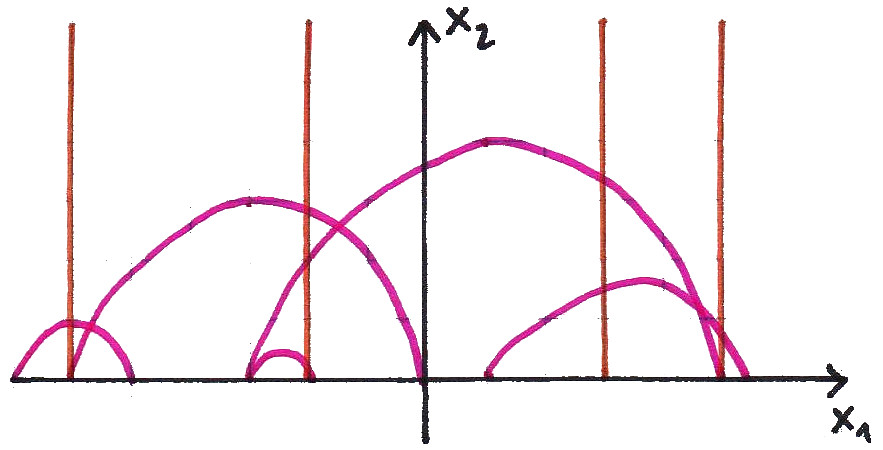
\includegraphics[width=.45\textwidth]{HyperbolischeGeraden}
    \caption{Sammlung verschiedener Geraden in der hyperbolischen Ebene}
  \end{figure}

  Leicht lässt sich zeigen, dass es wie in der euklidischen Geometrie auf der hyperbolischen Ebene eine Gerade zwischen zwei beliebigen Punkten gibt. Allerdings ist diese Gerade hier im Allgemeinen nicht eindeutig. Das Parallelen-Axiom gilt auf der hyperbolischen Ebene nicht, da hier zu gegebener Gerade \( g \) und Punkt \( P \) mehrere Geraden \( \widetilde{g_1}, \widetilde{g_2}, \dots \) gefunden werden können, sodass
  \begin{equation*}
    \widetilde{g_1} \cap g = \widetilde{g_2} \cap g = \cdots = \varnothing\text{.}
  \end{equation*}
\end{definition}

\section{Von Gauß zu Riemann}

\begin{minipage}{.475\textwidth}
  \begin{figure}[H]
    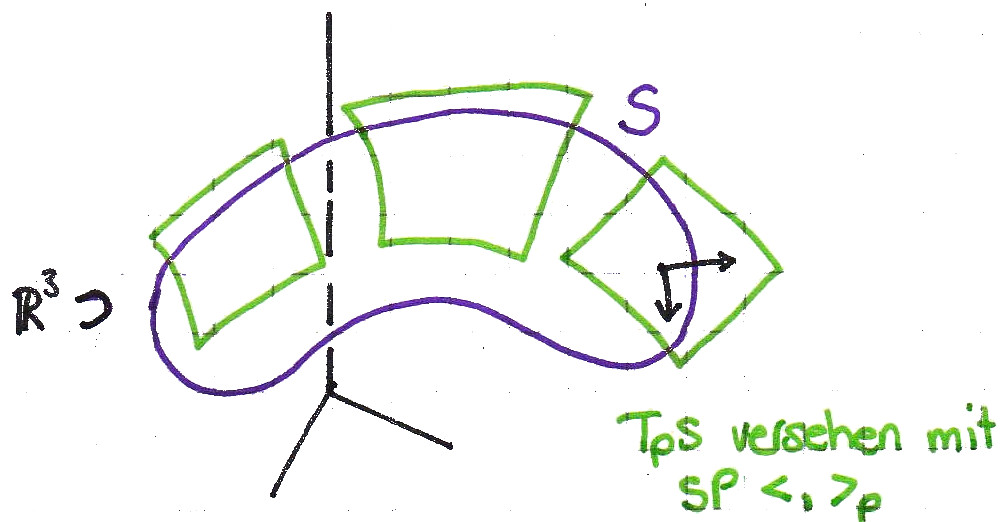
\includegraphics[width=\textwidth]{ModellGauss}
    \caption{Modell von Gauß (um 1827)}
  \end{figure}
\end{minipage}
\hfill
\begin{minipage}{.475\textwidth}
  \begin{figure}[H]
    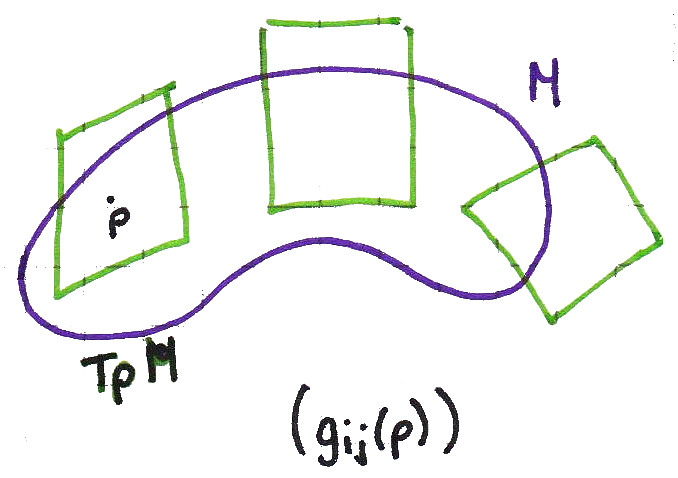
\includegraphics[width=.75\textwidth]{ModellRiemann}
    \vspace{1em}
    \caption{Modell von Riemann (um 1854).\enskip{} \( M \) ist hier eine differenzierbare Mannigfaltigkeit}
  \end{figure}
\end{minipage}

\  \\

Sei \( M \) eine \( m \)-dimensionale, differenzierbare Mannigfaltigkeit. Zu jedem \( p \in M \) definiert man abstrakt einen Tangentialraum \( T_p M \) wie folgt: \\
Tangentialvektoren sind Äquivalenzklassen von differenzierbaren Kurven durch \( p \in M \). Genauer: Ist \( (U, \phi) \) eine Karte um \( p \) und \( c_1, c_2: (-\epsilon, \epsilon) \to M \) mit \( c_1(0) = c_2(0) = p \), so ist
\begin{equation*}
  c_1 \sim c_2 \Leftrightarrow \frac{\text{d}}{\text{d}t}\vert_{t = 0} \phi \circ c_1(t) = \frac{\text{d}}{\text{d}t}\vert_{t = 0} \phi \circ c_2(t)\text{.}
\end{equation*}

\begin{figure}[H]
  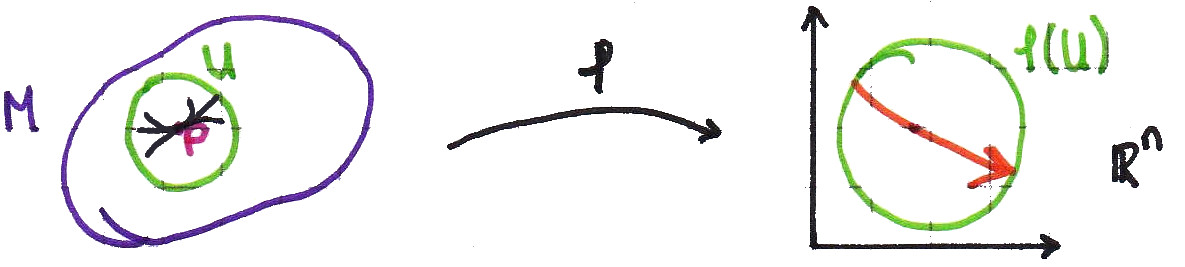
\includegraphics[width=.5\textwidth]{GaussZuRiemann}
\end{figure}

Man kann zeigen:
\begin{itemize}
  \item \( T_p M \) ist \( n \)-dimensionaler \( \R \)-Vektorraum.
  \item \( T_p M \) ist unabhängig von \( (U, \phi) \).
\end{itemize}

\begin{definition}[Riemannsche Metrik]
  Eine \term{Riemannsche Metrik} auf einer differenzierbaren Mannigfaltigkeit \( M \) ist eine Familie von Skalarprodukten \( \left\langle \cdot,\cdot \right\rangle_p \) auf \( T_p M \), die differenzierbar von \( p \) abhängt. \\
  Dieses Konzept verallgemeinert die erste Fundamentalform von Flächen in \( \R^3 \) auf \( n \)-dimensionale Mannigfaltigkeiten\footnote{Weiteres hierzu in der Vorlesung ``Differentialgeometrie''}.
\end{definition}

\begin{example}[Einfache Beispiele Riemannscher Mannigfaltigkeiten \( (M, \left\langle \cdot,\cdot \right\rangle) \)]
  \
  \begin{enumerate}
    \item \( M = U = \) offene Teilmenge von \( \R^n \). \\
      Hier ist \( T_p M = T_p U = T_p \R^n \cong \R^n \). \\
      Eine Riemannsche Metrik auf \( U \) ist gegeben durch eine Abbildung
      \begin{align*}
        g: U &\to \text{Sym}(n) = \text{ pos.\ definite, symmetrische } n \times n \text{-Matrizen} \\
        (u_1, \dots, u_n) &\mapsto (g_{ij}(u_1, \dots, u_n))
      \end{align*}

    \item Spezialfall für \( n = 2 \): \\
      \( U = \R^2 \), \( g_{ij}(x,y) = \left( \begin{smallmatrix}
        1 & 0 \\ 0 & 1
      \end{smallmatrix} \right) = \) konstant. \\
      Das ist genau die euklidische Geometrie aus Kapitel 1. Das heißt, dass riemannsche Metriken die euklidische Geometrie verallgemeinern.

    \item \( M = H^2 = \left \{ (x,y) \in \R^3 : y > 0 \right \} = \) obere Halbebene. \\
      Hier ist \( g_{ij}(x,y) = \frac{\delta_{ij}}{y^2} \), also \( (g_{ij}(x,y)) = \left( \begin{smallmatrix}
        \tfrac{1}{y^2} & 0 \\ 0 & \tfrac{1}{y^2}
      \end{smallmatrix} \right) \).
  \end{enumerate}
\end{example}

\begin{remark}[Wozu brauchen wir riemannsche Metriken?]
  \  \\
  Sei \( n = 2 \) und \( U \subset \R^2 \) offen. Für das Skalarprodukt von zwei Tangentialvektoren in \( T_{(u_1,u_2)}M \cong \R^2 \), \( a = (a_1, a_2) \) und \( b = (b_1,b_2) \) gilt:
  \begin{align*}
    g_{u_1 u_2}(a,b) &\coloneqq \left\langle a,b \right\rangle_{(u_1, u_2)} = \sum_{i,j = 1}^2 g_{ij}(u_1,u_2)a_i b_j \\
     &= g_{11}(u_1, u_2)a_1 b_1 + 2g_{12}(u_1, u_2)a_1 b_2 + 2g_{12}(u_1, u_2)a_2b_1 + g_{22}(u_1,u_2)a_2 b_2
  \end{align*}
  Insbesondere sind dadurch Längen von und Winkel zwischen Tangentialvektoren definiert:
  \begin{equation*}
    \left\Vert a \right\Vert_{(u_1, u_2)} = \sqrt{g(u_1,u_2)(a,a)} = \sqrt{\sum_{i,j = 1}^n g_{ij}(u_1,u_2)(a_i,a_j)}
  \end{equation*}

  \begin{minipage}{.65\textwidth}
    \begin{equation*}
      \cos \angle (a,b) = \frac{g(u_1,u_2)(a,b)}{\left\Vert a \right\Vert_{(u_1,u_2)} \left\Vert b \right\Vert_{(u_1,u_2)}}
    \end{equation*}
  \end{minipage}
  \hfill
  \begin{minipage}{.325\textwidth}
    \begin{figure}[H]
      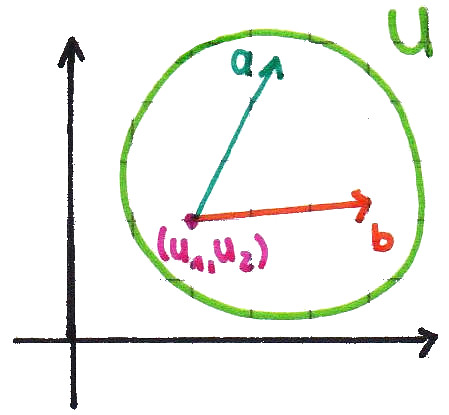
\includegraphics[width=.8\textwidth]{Tangentialvektoren}
    \end{figure}
  \end{minipage}
  \  \\

  Damit kann man wie in der Flächentheorie Längen von differenzierbaren Kurven, Flächeninhalt von Gebieten in \( U \) und allgemeiner alle Größen der inneren Geometrie für riemannsche Mannigfaltigkeiten verallgemeinern.
\end{remark}

\section{Ebene hyperbolische Geometrie}

\begin{definition}[Hyperbolische Länge]
  Sei
  \begin{equation*}
    H^2 = \left \{ (x,y) \in \R^2 : y > 0 \right \} = \left \{ z \in \C : \text{Im} z > 0 \right \}
  \end{equation*}
  die obere Halbebene mit der hyperbolischen riemannschen Metrik \( g_{ij} = \left( \begin{smallmatrix}
    \tfrac{1}{y^2} & 0 \\ 0 & \tfrac{1}{y^2}
  \end{smallmatrix} \right) \). \\
  Für eine differenzierbare Kurve 
  \begin{align*}
    c: [a,b] &\to H^2\text{,} \\
    t &\mapsto c(t) = (x(t),y(t))
  \end{align*}
  definieren wir die \term{hyperbolische Länge}:
  \begin{equation*}
    L_h(c) \coloneqq \int_a^b \left\Vert c' \right\Vert_H \text{d}t = \int_a^b \frac{\sqrt{{x'(t)}^2 + {y'(t)}^2}}{y(t)}\text{d}t\text{.}
  \end{equation*}
  Alternativ in komplexer Schreibweise:
  \begin{equation*}
    c(t) \coloneqq z(t) = x(t) + \i y(t) \quad \text{mit} \quad L_h(c) = \int_a^b \frac{\left\vert z'(t) \right\vert}{\text{Im} z(t)}\text{d}t\text{.}
  \end{equation*}
\end{definition}

\begin{example}
  Sei \( c: [a,b] \ni t \mapsto (0,t) \in H^2 \) das Stück der imaginären Achse zwischen \( \i a \) und \( \i b \). Dann gilt:
  \begin{equation*}
    L_h(c) = \int_a^b \frac{\sqrt{{x'(t)}^2 + {y'(t)}^2}}{y(t)}\text{d}t = \int_a^b \frac{1}{t}\text{d}t = \ln b - \ln a\text{.}
  \end{equation*}
  \emph{Bemerkung}: Es gilt \( \lim_{\i a \to \infty}L_h(c) = \infty \).
\end{example}

Wie die euklidische Ebene hat auch die hyperbolische Ebene viele Isometrien: \\
Betrachte dazu die spezielle lineare Gruppe \( \text{SL}(n,\R) \), also die Menge aller reellen \( 2 \times 2 \)-Metrizen mit Determinante \( 1 \), versehen mit der Matrizen-Multiplikation. \\

\begin{definition}[Möbius-Transformation]
  Für \( A = \left( \begin{smallmatrix}
    a & b \\ c & d
  \end{smallmatrix} \right) \in \text{SL}(n,\R) \) betrachten wir die \term{Möbius-Transformation}:
  \begin{equation*}
    T_A: H^2 \ni z \mapsto \frac{az + b}{cz + d} \in H^2\text{.}
  \end{equation*}
  \emph{Wohldefiniertheit}: Sei \( w = T_A(z) \). Es ist
  \begin{equation*}
    \text{Im}(w) = \frac{1}{2\text{i}}(w-\overline{w}) = \frac{1}{2\text{i}} \frac{z - \overline{z}}{\left\vert cz + d \right\vert} = \frac{\text{Im}(w)}{\left\vert cz + d \right\vert^2}\text{.}
  \end{equation*}
  Es gilt auch \( {(T_A)}^{-1} = T_{A^{-1}} \), also ist \( T_A \) bijektiv bzw. \( \det A = ad - bc \).
\end{definition}

\begin{lemma}[MT-Invarianz von Kurven]
  Die hyperbolische Länge einer differenzierbaren Kurve in \( H^2 \) ist invariant unter den Möbius-Transformationen
  \begin{equation*}
    \left \{ T_A : A \in \text{SL}(n,\R) \right \}
  \end{equation*}
  von \( H^2 \), also
  \begin{equation*}
    \forall A \in \text{SL}(n,\R) : L_h(T_a * c) = L_h(c)\text{.}
  \end{equation*}
  \begin{proof}
    Sei \( z(t) \) eine Kurve in \( H^2 \) und \( w(t) \coloneqq T_a(z(t)) \) die Bildkurve. Mit der Kettenregel und wegen \( \det A = ad - bc = 1 \) folgt:
    \begin{equation*}
      w' = \frac{\text{d}w}{\text{d}t} = \frac{\text{d}w}{\text{d}z} \frac{\text{d}z}{\text{d}t} = \frac{a(cz + d) - (az + b)c}{{(cz + d)}^2}z' = \frac{1}{{(cz + d)}^2}z' \text{.}
    \end{equation*}
    Weiter gilt:
    \begin{equation*}
      \text{Im}(w(t)) = \frac{1}{{(cz(t) + d)}^2}\text{Im}(z(t))
    \end{equation*}
    und somit ist
    \begin{equation*}
      \frac{\left\vert w'(t) \right\vert}{\text{Im}(w(t))} = \frac{\left\vert z'(t) \right\vert}{\left\vert {(cz + d)}^2 \right\vert} \frac{\left\vert cz + d \right\vert^2}{\text{Im}(z(t))} = \frac{\left\vert z'(t) \right\vert}{\text{Im}(z(t))}\text{.}
    \end{equation*}
    Die Behauptung folgt also aus der Definition von \( L_h \). \qed{}
  \end{proof}
\end{lemma}

\begin{definition}[Hyperbolische Längenmetrik]
  Analog zu \( \R^2 \), \( S^2 \) usw.\ definieren wir eine Längenmetrik
  \begin{equation*}
    d_h(p,q) \coloneqq \underset{c \in \Omega_{pq}}{\inf} L_h(c) \ \text{ mit } \ \Omega_{pq} \coloneqq \text{stückweise db. Kurven in \( H^2 \) zwischen \( p \) und \( q \).}
  \end{equation*}
\end{definition}

\begin{theorem}[Poincaré-Modell]
  \( (H^2, d_h) \) ist ein metrischer Raum.\footnote{Das ist das Poincaré-Modell der hyperbolischen Geometrie.}

  \begin{proof}
    Die Beweise von Symmetrie und Dreiecksungleichung sind analog zu vorhergehenden Beweisen von Metriken. Wir zeigen nur, dass
    \begin{equation*}
      d(p,q) = 0 \Leftrightarrow p = q
    \end{equation*}
    gilt.
    \begin{itemize}
      \item[\( \Leftarrow \)] Klar mit konstantem Weg.

      \begin{minipage}{.6\textwidth}
        \vspace{1em}
        \item[\( \Rightarrow \)] Zu zeigen: \( p \neq q \Rightarrow d(p,q) > 0 \). Sei dazu \( c:[a,b] \to H^2 \) eine stückweise differenzierbare Kurve. Weiter sei \( B_\delta(p) \) der euklidische Ball um \( p \) mit Radius \( \delta > 0 \) so klein, dass \( B_\delta \subset H^2 \) und \( q \not \in B_\delta(p) \).        
      \end{minipage}
      \hfill
      \begin{minipage}{.375\textwidth}
        \begin{figure}[H]
          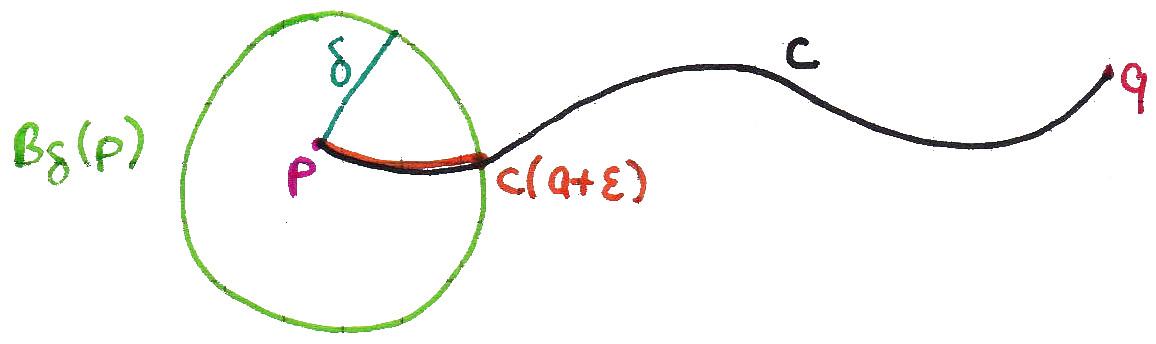
\includegraphics[width=.8\textwidth]{PoincareModell}
        \end{figure}
      \end{minipage}
      \  \\

      Dann existiert ein maximales \( \epsilon > 0 \), sodass
      \begin{equation*}
        c([a, a + \epsilon]) \subset B_\delta(p)\text{.}
      \end{equation*}
      Insbesondere ist \( \text{Im}(c(t)) \leq \text{Im}(p) + \delta \) für \( t \in [a, a + \epsilon] \). Damit folgt
      \begin{align*}
        L_h(c) &= \int_a^b \frac{\left\Vert c'(t) \right\Vert}{\text{Im}(c(t))}\text{d}t \geq \int_a^{a + \epsilon} \frac{\left\Vert c'(t) \right\Vert}{\text{Im}(c(t))}\text{d}t \geq \frac{1}{\text{Im}(p) + \delta} \underbrace{\int_a^{a + \epsilon}\left\Vert c'(t) \right\Vert \text{d}t}_{\geq \delta} \\
        &\geq \frac{\delta}{\text{Im}(p) + \delta} > c\text{.}
      \end{align*}
      Daraus folgt die Behauptung, da \( c \) beliebig ist. \qed{}
    \end{itemize}
  \end{proof}
\end{theorem}

\begin{theorem}
  \
  \begin{enumerate}
    \item Die Möbius-Transformationen \( \left \{ T_A : A \in \text{SL}(2,\R) \right \} \) sind Isometrien des Metrischen Raums \( (H^2, d_h) \) (also der hyperbolischen Ebene).
    \item Die hyperbolische Ebene \( (H^2, d_h) \) ist homogen, also existiert für \( p,q \in H^2 \) eine Isometrie \( T_A \), sodass \( T_A(p) = q \).
  \end{enumerate}

  \begin{proof}
    \
    \begin{enumerate}
      \item Ein früheres Lemma besagt, dass \( L_h(T_A \circ c) = L_h(c) \). Der Beweis folgt damit aus der Definition von \( d_h \).

      \item Es genügt zu zeigen, dass zu gegebenem \( z = x + \i y \in H^2 \) ein \( A \in \text{SL}(2,\R) \) existiert, sodass \( T_A(i) = z \). Dann gilt nämlich für \( w = T_B(\i) \) und \( z = T_A(\i) \), dass \( z = T_A \circ T_B^{-1}(w) \). Setze dazu
      \begin{equation*}
        A \coloneqq \underbrace{\begin{pmatrix}
          1 & x \\ 0 & 1
        \end{pmatrix}}_{A_1}\underbrace{\begin{pmatrix}
          \sqrt{y} & 0 \\ 0 & \sqrt{y}^{-1}
        \end{pmatrix}}_{A_2}\text{.}
      \end{equation*}
      Dann ist
      \begin{align*}
        T_{A_1}(\i) &= \frac{\sqrt{y}\i + 0}{0\i + \sqrt{y}^{-1}} = \i y \quad \text{und} \\
        T_{A_2}(\i) &= \frac{1\i y + x}{0\i y + 1} = x + \i y = z\text{.}
      \end{align*}
      Daraus folgt die Behauptung. \qed{}
    \end{enumerate}
  \end{proof}
\end{theorem}

\begin{remark}
  \
  \begin{enumerate}

    \begin{minipage}{.6\textwidth}
      \item Sei \( A = \left( \begin{smallmatrix}
        \sqrt{\lambda} & 0 \\ 0 & \frac{1}{\sqrt{\lambda}}
      \end{smallmatrix} \right) \in \text{SL}(2,\R) \), \( \lambda > 0 \). Dann ist
      \begin{equation*}
        T_s(z) = \frac{\sqrt{\lambda}z + 0}{0z + \frac{1}{\sqrt{\lambda}}} = \lambda z
      \end{equation*}
      eine Streckung.
      \vspace{1em}
    \end{minipage}
    \hfill
    \begin{minipage}{.375\textwidth}
      \begin{figure}[H]
        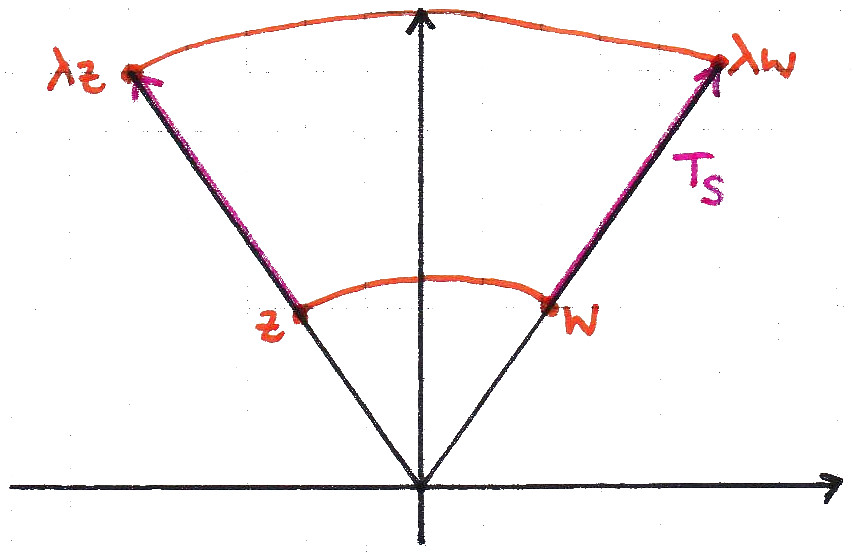
\includegraphics[width=.8\textwidth]{KuerzesteVerbindungskurvenHyperbolisch}
      \end{figure}
    \end{minipage}
    Die kürzesten Verbindungsstrecken von \( z \) zu \( w \) und \( \lambda z \) zu \( \lambda w \) sind also hyperbolisch gleich lang, da Streckungen Isometrien in \( H^2 \) sind.\footnote{In der euklidischen Ebene sind Streckungen \emph{keine} Isometrien!}


    \item Kürzeste Verbindungen: Einheitsquadrate
    \begin{figure}[H]
      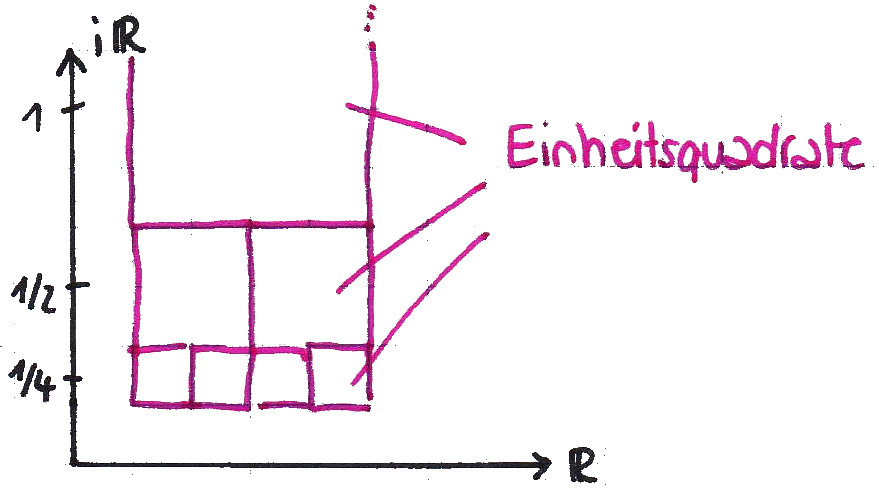
\includegraphics[width=.4\textwidth]{Einheitsquadrate}
    \end{figure}
  \end{enumerate}
\end{remark}

\section{Geodätische}

\begin{theorem}[Geodätische]
  Kürzeste Verbindungskurven (\term{Geodätische}) zwischen Punkten von \( (H^2, d_h) \) sind geeignete parametrisierte Halbkreise und Geraden orthogonal zur reellen Achse.

  Solche Halbkreise haben ihr Zentrum auf der reellen Achse.
\end{theorem}

Für den Beweis dieses Satzes benötigen wir folgendes Lemma:

\begin{lemma}
  Sei \( K \) ein euklidischer Halbkreis oder eine Halbgerade, welche die reelle Achse in einem Punkt \( \alpha \) orthogonal schneidet. Dann ist
  \begin{equation*}
    T(z) = {(z - \alpha)}^{-1} + \beta
  \end{equation*}
  eine Möbius-Transformation (also \( T = T_A \) für ein \( A \in \text{SL}(2,\R) \)) und bildet \( K \) für ein geeignetes \( \beta \) auf die imaginäre Achse ab. \\
  \  \\
  \emph{Hinweis}: \( T = T_\beta \circ J \circ T_\alpha \), wobei \( J(z) = -\frac{1}{z} \) und generell ist \( T_\gamma(t) = t + \gamma \) eine Translation um \( \gamma \).
\end{lemma}

Wir beweisen nun den Satz.

\begin{proof}
  Seien \( z_1 \), \( z_2 \) zwei Punkte in \( H^2 \). Gesucht ist die kürzeste Verbindung zwischen \( z_1 \) und \( z_2 \).
  \begin{enumerate}
    \item \textbf{Fall 1}: \( z_1 = a\i \), \( z_2 = b\i \) mit \( b > a \).

    Ist \( c : [0,1] \ni t \mapsto c(t) = (x(t), y(t)) \in H^2 \) ein Testweg zwischen \( a\i \) und \( b\i \), so ist
    \begin{align*}
      L_h(c) &= \int_0^1 \frac{\sqrt{x'^2 + y'^2}}{y(t)}\text{d}t \geq \int_0^1 \frac{\sqrt{y'^2}}{y(t)}\text{d}t \geq \int_0^1 \frac{\left\vert y' \right\vert}{y(t)}\text{d}t \geq \int_0^1 \frac{\frac{\text{d}y}{\text{d}t}}{y(t)}\text{d}t \\
       &= \int_a^b \frac{\text{d}y}{y} = \ln(b) - \ln(a)\text{.}
    \end{align*}
    Also ist die hyperbolische Länge des Geradensegments auf der imaginären Achse zwischen \( z_1 \) und \( z_2 \). \qed{}

    \item \textbf{Fall 2}: \( z_1, z_2 \in H^2 \) beliebig. Dann existiert genau eine Gerade (falls \( \text{Re}(z_1) = \text{Re}(z_2) \)) bzw ein Halbkreis \( k \) mit Zentrum auf der reellen Achse, der \( z_1 \) und \( z_2 \) trifft.

    Nach dem Lemma existiert eine Möbius-Transformation --- also eine Isometrie --- \( T_A \) von \( H^2 \), sodass \( T_A(K) = \) imaginäre Achse. Da \( T_A \) Abstände erhält, bildet sie kürzeste Verbindungen auf kürzeste Verbindungen ab. Daraus folgt die Behauptung. \qed{}
  \end{enumerate}
\end{proof}

\begin{corollary}
  Je zwei Punkte \( p,q \in H^2 \) können durch eine eindeutige Geodätische verbunden werden und der hyperbolische Abstand ist genau gleich der hyperbolischen Länge des eindeutigen geodätischen Segments zwischen \( p \) und \( q \).
\end{corollary}

\section{Nochmals Gauß-Bonnet}

\begin{definition}[Hyperbolischer Flächeninhalt]
  Der \term{hyperbolische Flächeninhalt} für \( A \subset H^2 \) ist
  \begin{equation*}
    \mu(A) \coloneqq \iint_A \sqrt{\det(g_{ij}(z))}\text{d}x\text{d}y = \iint_A \frac{1}{y^2} \text{d}x\text{d}y \leq x \quad \text{(falls das Integral existiert).}
  \end{equation*}  
\end{definition}

\begin{theorem}[Flächeninhalt invariant unter Isometrien]
  Der hyperbolische Flächeninhalt ist invariant unter Isometrien (also Möbius-Transformationen). Falls für \( A \subset H^2 \) \( \mu(A) \) existiert ung \( T_B \) eine Möbius-Transformation für \( B \in \text{SL}(2,\R) \) ist, so gilt
  \begin{equation*}
    \mu(T_B(A)) = \mu(A)\text{.}
  \end{equation*}

  \begin{proof}
    Sei \( z = x + \i y \), \( T(z) = \frac{dz + b}{cz + d} \) (\( a,b,c,d \in \R \), \( ad - bc = 1 \)) und \( w \coloneqq T(z) = u+\i v \). Es gilt für die Jacobi-Determinante:
    \begin{equation*}
      \frac{\partial(u,v)}{\partial(x,y)} = \frac{\partial u}{\partial x} \frac{\partial v}{\partial y} - \frac{\partial u}{\partial y} \frac{\partial v}{\partial x} = \frac{1}{\left\vert cz + d \right\vert^4}\text{.}
    \end{equation*}
    Also gilt mit der Transformation für Integrale:
    \begin{equation*}
      \mu(T(A)) = \iint_{T(A)} \frac{\text{d}u\text{d}v}{v^2} = \iint_A \frac{\partial(u,v)}{\partial (x,y)} \frac{\text{d}x\text{d}y}{v^2} = \iint_A \frac{1}{\left\vert cz + d \right\vert^4} \frac{\left\vert cz + d \right\vert^4}{y} \text{d}x\text{d}y = \mu(A)\text{.}
    \end{equation*} \qed{}
  \end{proof}
\end{theorem}

\begin{definition}[Hyperbolisches Polygon]
  Ein \term{hyperbolisches Polygon} mit \( n \) Seiten ist eine abgeschlossene Teilmenge von \( \overline{H^2} \coloneqq H^2 \cup \left( \R \cup \left \{ \infty \right \} \right) \), die durch \( n \) geodätische Segmente (\( \cong \) Seiten) begrenzt ist. Wenn sich \( 2 \) Segmente in genau einem Punkt schneiden, so heißt der Schnittpunkt \term{Ecke} einer Polygons. Wir lassen Ecken im ``Rand und Unendlichen'' \( \R \cup \left \{ \infty \right \} \) zu, aber keine Segmente.
  \begin{figure}[H]
    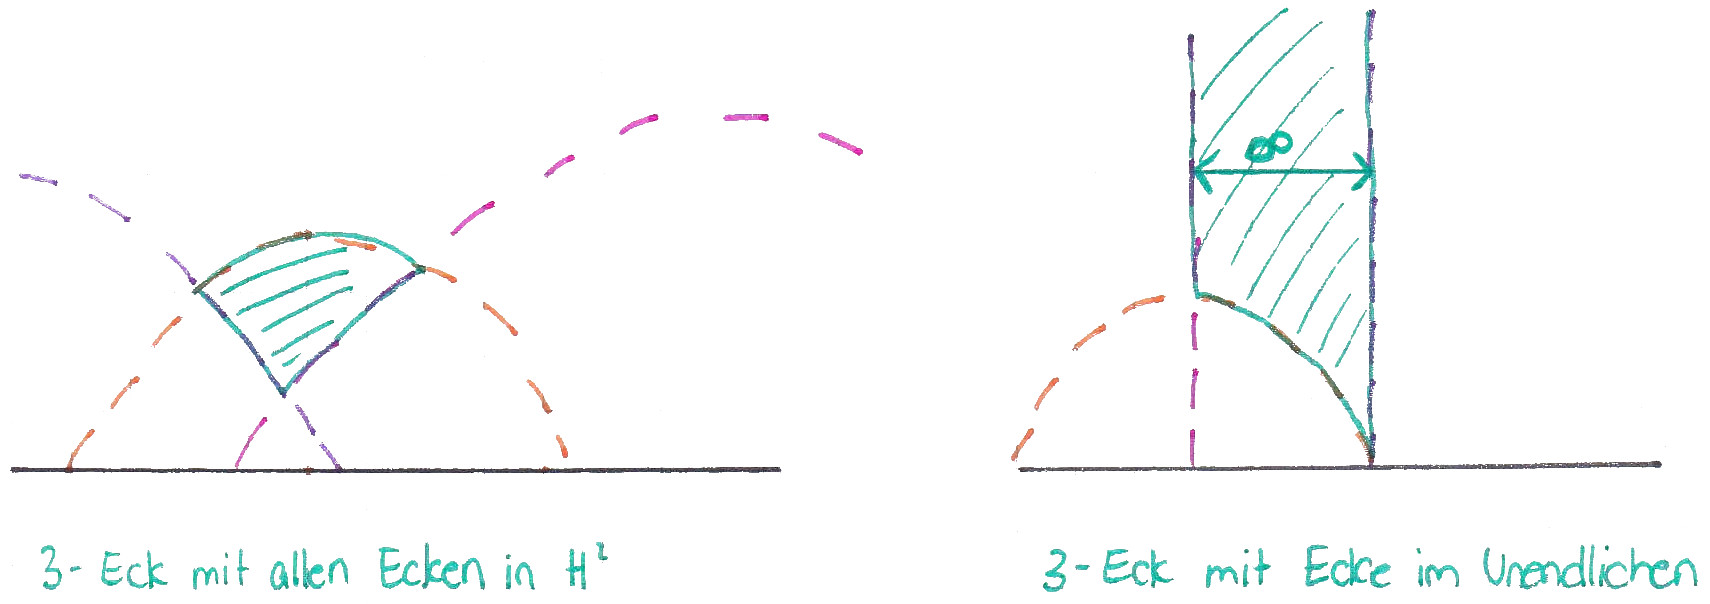
\includegraphics[width=.8\textwidth]{HyperbolischeDreiecke}
    \caption{Zwei verschiedene Dreiecke im Hyperbolischen}
  \end{figure}
\end{definition}

\begin{remark}[Hyperbolische Winkelmessung]
  Die Messung von Winkeln erfolgt im Hyperbolischen über Tangenten an Kurven. Seien dazu \( a, b \in T_B H^2 \) zwei Tangentialvektoren an die geodätischen Segmente durch den Punkt \( z \):
  \begin{equation*}
    \cos \measuredangle_\text{hyp}(a,b) \overset{\mathclap{\substack{\text{Def. Riemann-} \\ \text{Metrik} \\ \ }}}{=} \frac{\left\langle a,b \right\rangle_z}{\left\Vert a \right\Vert_z \left\Vert b \right\Vert_z} = \frac{\frac{\left\langle a,b \right\rangle_\text{euk}}{\text{Im}{(z)}^2}}{\frac{\left\Vert a \right\Vert_{\text{euk}}}{\text{Im}(z)} \frac{\left\Vert b \right\Vert_{\text{euk}}}{\text{Im}(z)}} = \frac{\left\langle a,b \right\rangle_\text{euk}}{\left\Vert a \right\Vert_\text{euk} \left\Vert b \right\Vert_\text{euk}} = \cos \measuredangle_\text{euk}(a,b)
  \end{equation*}
  Also entspricht der hyperbolische Winkel dem euklidischen Winkel.
\end{remark}

\begin{theorem}[Gauß-Bonnet für hyperbolische Ebene]
  Der Flächeninhalt einer hyperbolischen Dreiecks ist durch die Winkel vollständig bestimmt: \\
  Sei \( \triangle \) ein hyperbolisches Dreieck mit den Winkeln \( \alpha, \beta, \gamma \). Dann gilt:
  \begin{equation*}
    \mu(\triangle) = \pi - \alpha - \beta - \gamma \leq \pi\text{.}
  \end{equation*}
\end{theorem}

\begin{remark}[Bemerkungen zum Satz]
  \ 
  \begin{enumerate}
    \item Ein analoger Satz gilt \textbf{nicht} in der euklidischen Ebene. Ein gleichseitiges Dreieck kann beliebig groß werden, die Innenwinkel bleiben trotzdem alle gleich.
    \item Für nicht entartete Dreiecke gilt:
    \begin{equation*}
      0 < \mu(\triangle) = \pi - (\alpha + \beta + \gamma) \Leftrightarrow \alpha + \beta + \gamma < \pi\text{.}
    \end{equation*}

    \begin{minipage}{.475\textwidth}
      \item Es existieren in der hyperbolischen Ebene Dreiecke mit \( \mu(\triangle) = \pi \). Das ist der Fall, wenn alle Ecken in \( \R \cup \left \{ \infty \right \} \) sind.
    \end{minipage}
    \hfill
    \begin{minipage}{.475\textwidth}
      \begin{figure}[H]
        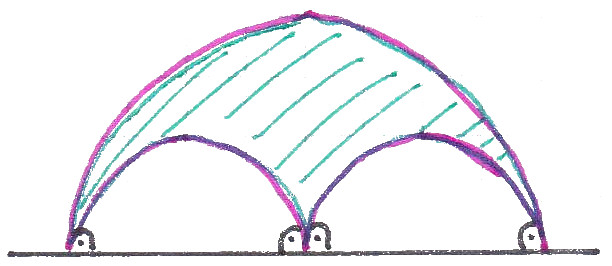
\includegraphics[width=.7\textwidth]{SpeziellesHyperbolischesDreieck}
        \caption{Dreieck mit \( \mu(\triangle) = \pi \)}
      \end{figure}
    \end{minipage}
    \begin{proof}
      \  \\
      \begin{minipage}{.475\textwidth}
        \textbf{Fall 1}: Eine Ecke \( E \) liegt in \( \R \cup \left \{ \infty \right \} \), der Winkel bei \( E \) ist also \(  0 \). Durch eine Möbius-Transformation \( T_A \) mit \( A \in \text{SL}(2,\R) \) können wir erreichen, dass \( E \) nach \( \infty \) abgebildet wird (Ansatz: \( T(z) = \frac{az + b}{cz + d} \), \( T(z) = \infty \), \( ab - cd = 1 \), Gleichungssystem).
      \end{minipage}
      \hfill
      \begin{minipage}{.475\textwidth}
        \begin{figure}[H]
          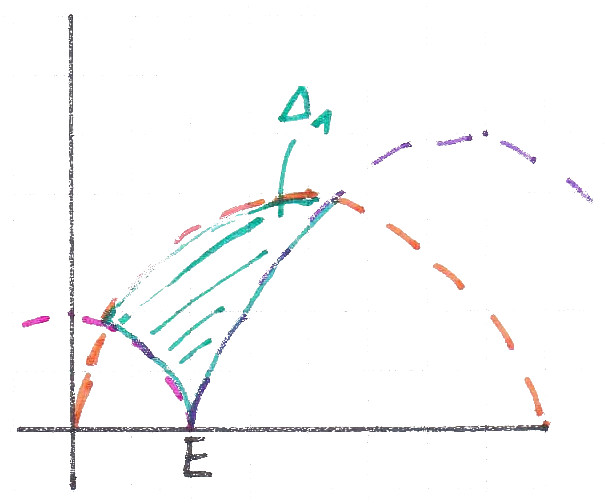
\includegraphics[width=.6\textwidth]{HyperbolischesDreieckTransformieren1}
        \end{figure}
      \end{minipage}

      \begin{minipage}{.475\textwidth}
        Dann hat man ein Dreieck der Gestalt \( \triangle_2 \). Dabei ändert sich der Flächeninhalt nicht. Es genügt also den Fall zu betrachten, dass \( 2 \) Seiten des Dreiecks vertikal sind.
      \end{minipage}
      \hfill
      \begin{minipage}{.475\textwidth}
        \begin{figure}[H]
          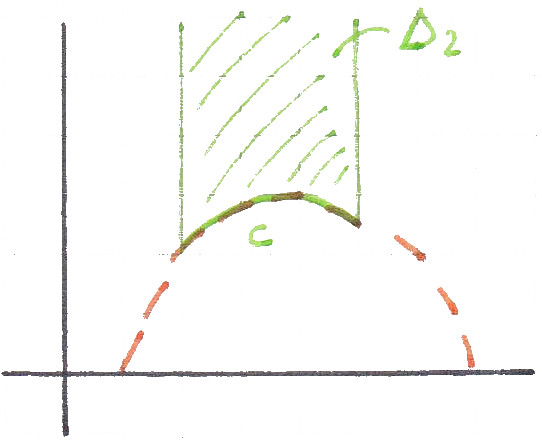
\includegraphics[width=.6\textwidth]{HyperbolischesDreieckTransformieren2}
        \end{figure}
      \end{minipage}


      Durch eine weitere Möbius-Transformation der Form
      \begin{equation*}
        z \mapsto z + k \ (k \in \R) \quad \text{und} \quad z \mapsto \lambda z \ (\lambda > 0)
      \end{equation*}
      können wir die Seite \( c \) auf den Einheitskreis um \( 0 \) abbilden --- wieder ohne Änderung des Flächeninhalts.

      \begin{figure}[H]
        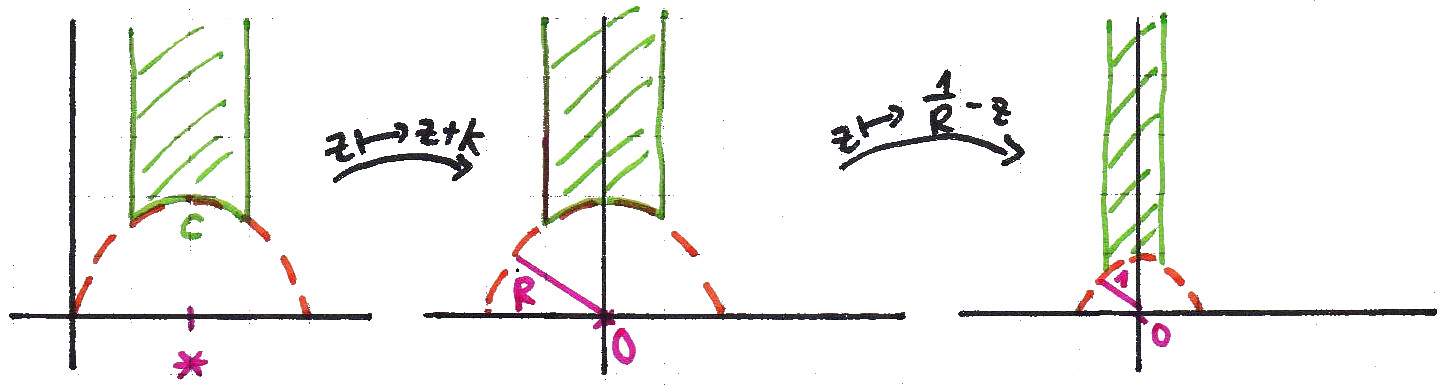
\includegraphics[width=.6\textwidth]{HyperbolischesDreieckTransformierenUebersicht}
        \caption{Abbildung auf den Einheitskreis um \( 0 \)}
      \end{figure}

      \begin{minipage}{.475\textwidth}
        Wir haben also ohne Einschränkung folgende Situation: \( \measuredangle(AOE) = \alpha \), \( \measuredangle(BOD) = \beta \) (da die Geraden paarweise senkrecht sind).
      \end{minipage}
      \hfill
      \begin{minipage}{.475\textwidth}
        \begin{figure}[H]
          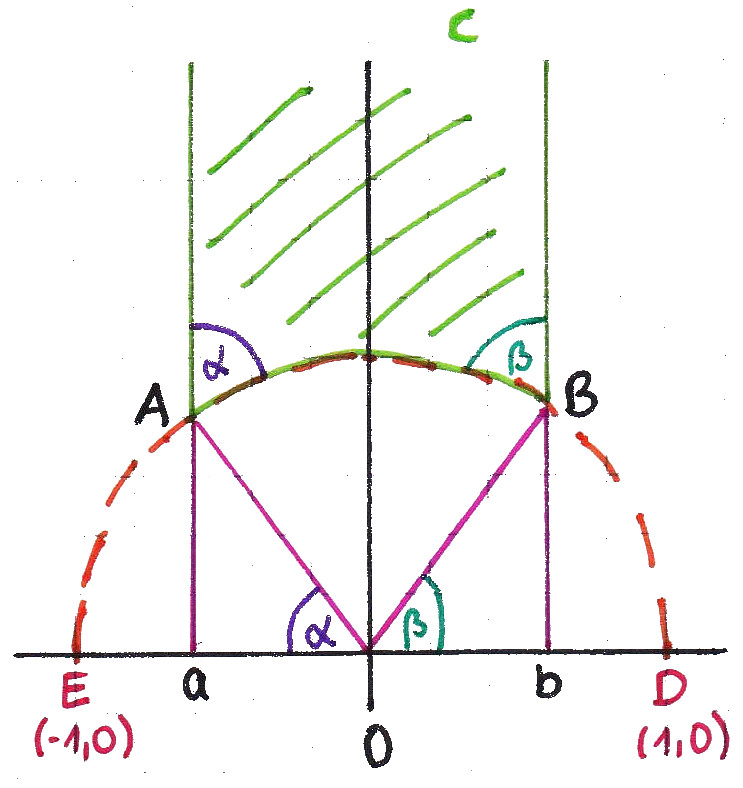
\includegraphics[width=.6\textwidth]{HyperbolischesDreieckTransformierenWinkel}
        \end{figure}
      \end{minipage}

      Und nun ist
      \begin{equation*}
        \mu(\triangle) = \iint_A \frac{\text{d}x\text{d}y}{y^2} = \int_a^b \text{d}x \int_{\sqrt{1-x^2}}^\infty \frac{\text{d}y}{y^2} = \int_a^b \frac{\text{d}x}{\sqrt{1-x^2}} = \int_{\pi - \alpha}^\beta \frac{-\sin \theta}{\sin \theta}\text{d}\theta = \pi - \alpha - \beta\text{.}
      \end{equation*}

      \textbf{Fall 2}: \( \triangle \) hat keine Ecken in \( \R \cup \left \{ \infty \right \} \). Wir führen diesen Fall auf den ersten Fall zurück, indem wir eine Ecke ins Unendliche führen. Dazu verlängern wir eine Seite:

      \begin{minipage}{.475\textwidth}
        \begin{figure}[H]
          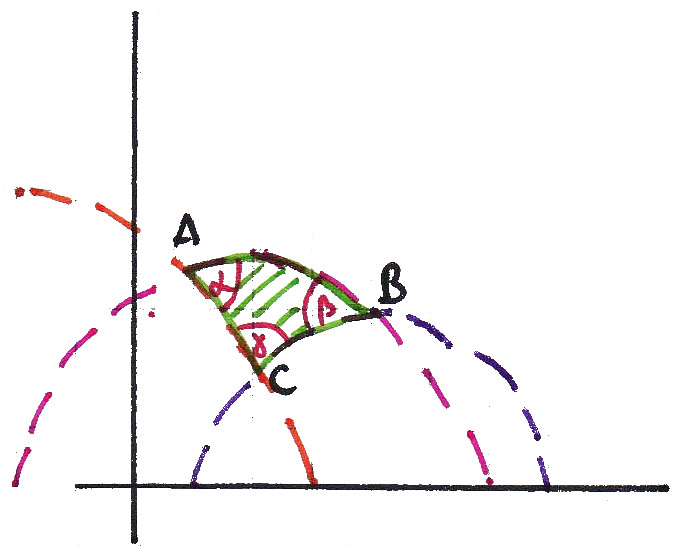
\includegraphics[width=.7\textwidth]{HyperbolischesDreieckTransformieren3}
        \end{figure}
      \end{minipage}
      \hfill
      \begin{minipage}{.475\textwidth}
        \begin{figure}[H]
          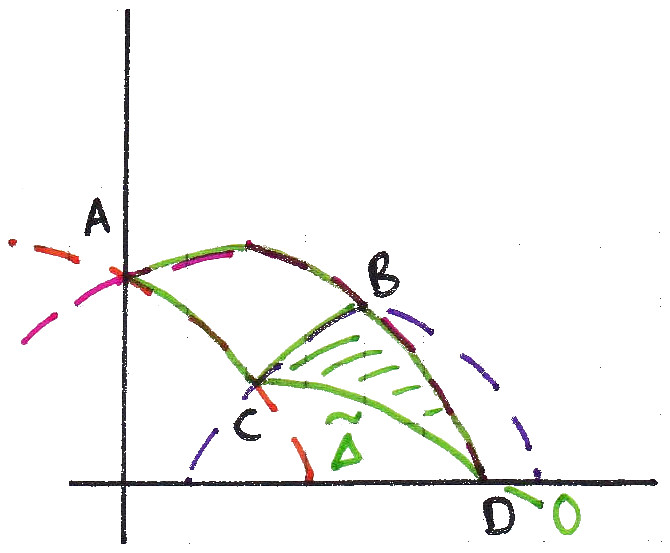
\includegraphics[width=.7\textwidth]{HyperbolischesDreieckTransformieren4}
        \end{figure}
      \end{minipage}
      \  \\

      Das neue Dreieck \( BCD \eqqcolon \widetilde{\triangle} \) mit Winkeln \( \delta, 0, \pi - \beta \) entsteht. Nun ist
      \begin{equation*}
        \mu(\triangle) = \underbrace{\mu(ACD)}_{= \triangle \cup \widetilde{\triangle}} - \mu(\widetilde{\triangle}) \overset{\text{F1}}{=} \left( \pi - \alpha - (\gamma + \delta) \right) - \left( \pi - \delta - (\pi - \beta) \right) = \pi - \alpha - \beta - \gamma\text{.}
      \end{equation*} \qed{}
    \end{proof}
  \end{enumerate}
\end{remark}

\section{Einheitsmodell für die hyperbolische Ebene, Krümmung}

Sei \( D^2 \coloneqq \left \{ (x,y) \in \R^2 : x^2 + y^2 < 1 \right \} = \left \{ z \in \C : \left\vert z \right\vert < 1 \right \} \) die (offene) \term{Einheitsscheibe} (eine offene Untermannigfaltigkeit von \( \R^2 \)). Die Abbildung
\begin{equation*}
  M : H^2 \to D^2\text{,} \ z \mapsto \frac{\i z + 1}{z + \i}
\end{equation*}
ist eine injektive Abbildung von \( H^2 \) nach \( D^2 \).\footnote{siehe Übungsblatt 11.4}

Wir definieren eine Metrik auf \( D^2 \) durch
\begin{equation*}
  d_h^\ast(z,w) \coloneqq d_h\left( M^{-1}(z),M^{-1}(w) \right)\text{.}
\end{equation*}
Wir verlangen also per Definition, dass \( M \) eine Isometrie ist.

\begin{remark}
  \( d_h^\ast \) ist die von der riemannschen Metrik
  \begin{equation*}
    \left( g_{ij}(z) \right) \coloneqq \left( \frac{4\delta_{ij}}{{\left( 1-\left\vert z \right\vert^2 \right)}^2} \right) = \begin{pmatrix}
      \frac{4}{{\left( 1-\left\vert z \right\vert^2 \right)}^2} & 0 \\
      0 & \frac{4}{{\left( 1-\left\vert z \right\vert^2 \right)}^2}
    \end{pmatrix}
  \end{equation*}
  auf \( D^2 \) induzierte Längenmetrik, für die gilt:
  \begin{equation*}
    L_h^\ast(M(c)) = L_h(c)\text{.}
  \end{equation*}
\end{remark}

\begin{theorem}
  \
  \begin{enumerate}
    \item Die euklidischen Rotationen um \( O \in D^2 \) sind Isometrien von \( (D^2, d_h^\ast) \).
    \item Für \( 0 < r < 1 \) gilt
    \begin{equation*}
      d_h^\ast(0,\i r) = \ln\frac{1+r}{1-r}\text{.}
    \end{equation*}
  \end{enumerate}
  \begin{proof}
    \
    \begin{enumerate}
      \item Wir benutzen die riemannsche Metrik auf \( D^2 \). Sei \( z = x(t) + \i y(t) \) eine Kurve in \( D^2 \) und \( R(z(t)) \) die Bildkurve einer Rotation:
      \begin{equation*}
        R = \begin{pmatrix}
          \cos \theta & - \sin \theta \\
          \sin \theta & \cos \theta
        \end{pmatrix}\text{,}\quad \theta \in [0,2\pi]\text{.}
      \end{equation*}
      Dann gilt:
      \begin{equation*}
        \left\vert R(z(t)) \right\vert = \left\vert z(t) \right\vert \quad \text{und} \quad R(z(t))' = R(z'(t))\text{,}
      \end{equation*}
      da \( R \) linear ist. Also gilt:
      \begin{equation*}
        L_{h^\ast}(R(z(t))) = \int_a^b \frac{2\left\vert (R(z(t)))' \right\vert\text{d}t}{1-\left\vert R(z(t)) \right\vert^2} = \int_a^b \frac{2\left\vert z'(t) \right\vert\text{d}t}{1-\left\vert z(t) \right\vert^2} = L_{h^\ast}(z(t))\text{.}
      \end{equation*}
      Daraus folgt die Behauptung. \qed{}

      \begin{minipage}{.65\textwidth}
        \item Eine Abschätzung der Länge einer beliebigen Kurve in \( D^2 \), die \( 0 \) und \( \i r \) verbindet, zeigt
        \begin{align*}
          L_{h^\ast}(c) &= \int_0^r \frac{2\text{d}t}{1-t^2} = \ln\left( \frac{1+r}{1-r} \right) = 2\text{arctanh}(r) \quad \text{und} \\
          h^\ast &= \text{Länge des Geraden-Segments } [0,\i r] = \ln\left( \frac{1+r}{1-r} \right)\text{.}
        \end{align*}
      \end{minipage}
      \hfill
      \begin{minipage}{.325\textwidth}
        \begin{figure}[H]
          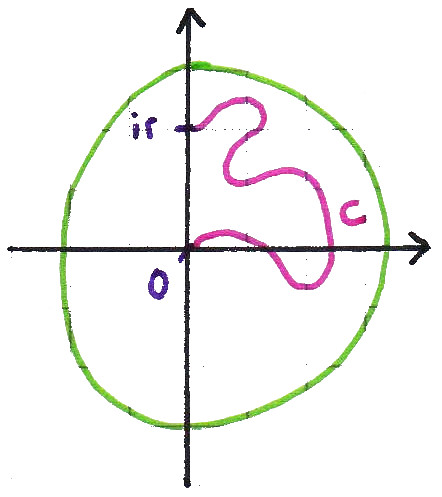
\includegraphics[width=.8\textwidth]{HyperbolischeKurve}
        \end{figure}
      \end{minipage}
      \qed{}
    \end{enumerate}
  \end{proof}
\end{theorem}

\begin{deduction}
  \
  \begin{enumerate}
    \item Radiale Segmente durch \( 0 \) sind Geodätische in \( D^2 \).

    \emph{Ergänzung}: Man kann zeigen, dass Geodätische in \( D^2 \) Kreis-Stücke (in \( D^2 \)) sind, die den Randkreis orthogonal schneiden.

    \item Die hyperbolischen Kreise in \( D^2 \) um \( 0 \) mit hyperbolischem Radius \( \rho \),
    \begin{equation*}
      S_\rho(0) \coloneqq \left \{ z \in D^2 : d_h^\ast(0,z) = \rho \right \}\text{,}
    \end{equation*}
    sind genau die euklidischen Kreise um \( 0 \) mit euklidischem Radius \( r \) so, dass
    \begin{equation*}
      \rho = 2 \text{arctanh}(r) \Leftrightarrow r = \text{tanh}\frac{\rho}{2}\text{.}
    \end{equation*}
  \end{enumerate}
\end{deduction}

\begin{remark}[Anwendung]
  Die hyperbolische Länge eines hyperbolischen Kreises mit hyperbolischem Radius \( \rho \) (Zentrum \( 0 \)) ist
  \begin{equation*}
    L_{h^\ast}(S_\rho(0)) = 2\pi\text{sinh}(\rho) \ (\approx 2\pi e^\rho)\text{.}
  \end{equation*}

  \begin{proof}
    Nach obigem Satz ist dieser Kreis wie folgt durch eine Kurve parametrisiert:
    \begin{equation*}
      z(t) = R(t) \i r = \begin{pmatrix}
        \cos t & -\sin t \\
        \sin t & \cos t
      \end{pmatrix}\begin{pmatrix}
        0 \\ r
      \end{pmatrix} = r\cos t + \i r \sin t\text{,}\quad t \in [0,2\pi]\text{,} \ r = \text{tanh}\frac{\rho}{2}\text{.}
    \end{equation*}
    Es gilt dann:
    \begin{align*}
      L_{h^\ast}(S_\rho(0)) &= \int_0^{2\pi} \frac{2\left\vert z'(t) \right\vert\text{d}t}{1-\left\vert z(t) \right\vert^2} = \int_0^{2\pi}\frac{2r}{1-r^2}\text{d}t = 2\pi \frac{2r}{1-r^2} = 2\pi \frac{2 \text{tanh}\frac{\rho}{2}}{1-\text{tanh}\frac{\rho}{2}} \\
      &= 2\pi \frac{2\text{sinh}\frac{\rho}{2}}{\text{cosh}\frac{\rho}{2}}\text{cosh}^2\frac{\rho}{2} = 2\pi * \underbrace{2\text{sinh}\frac{\rho}{2}\text{cosh}\frac{\rho}{2}}_{= \text{sinh}\rho} = 2\pi \text{sinh}(\rho)\text{.}
    \end{align*} \qed{}
  \end{proof}
\end{remark}

\begin{remark}
  \
  \begin{enumerate}
    \item Euklidische Länge eines euklidischen Kreises um \( 0 \) mit euklidischem Radius \( \rho \) ist \( 2\pi\rho \).
    \item Sphärische Länge eines sphärischen Kreises um \( N \) mit sphärischem Radius \( \rho \) ist \( 2\pi\underbrace{\sin \rho}_{< \rho} \).
  \end{enumerate}
  \emph{Erinnerung}: Gauß-Krümmung war definiert für reguläre Flächen in \( \R^3 \): \( K(p) = \frac{\det I_p}{\det II_p} \). Weiter gilt nach Gauß:

  \( K \) ist unabhängig von der Einbettung der Fläche in \( \R^3 \) (ist also Größe der inneren Geometrie).
\end{remark}

\begin{definition}[Krümmung]
  Wir definieren die (Gauß-)\term{Krümmung} für einen Längenraum durch die Bertrand-Puiseaux-Formel:
  \begin{equation*}
    K(p) \coloneqq \lim_{\rho \to 0} \frac{3}{\pi p^3}\left( 2\pi\rho - L\left( S_\rho(0) \right) \right)\text{.}
  \end{equation*}
\end{definition}

\begin{theorem}
  Die Gauß-Krümmung von \( D^2 \) (\( \cong H^2 \)) ist konstant \( -1 \).

  \begin{proof}
    \
    \begin{align*}
      L_{h^\ast}(S_\rho(0)) &= 2\pi\sin\rho = 2\pi\left( \rho + \frac{1}{3!}p^3 + \frac{1}{5!}p^5 + \cdots \right) \\
       &\Rightarrow K(0) = \lim_{\rho \to 0} \frac{3}{\pi \rho^3}\left( 2\pi\rho - 2\pi\rho - \left( \frac{2\pi}{3!}\rho^3 \right) - \cdots \right) = -1\text{.}
    \end{align*}
    \( (D^2, d_h^\ast) \) ist isometrisch zu \( (H^2, d_h) \). \( (H^2, d_h) \) ist homogen, also auch \( (D^2, d_h^\ast) \).

    \( \Rightarrow K(p) = K(0) \) für alle \( p \in D^2 \). \qed{}
  \end{proof}
\end{theorem}

\begin{remark}[Ausblick --- moderne hyperbolische Geometrie]
  \
  \begin{enumerate}
    \item Struktur von \( 3 \)-Mannigfaltigkeiten --- Geometrisierungsvermutung\footnote{Thurston, um 1970}.

      \( \Rightarrow 8 \) Geometrien als Bausteine, hyperbolische Geometrien sind hier die wichtigsten. Verifikation in der berühmten Arbeit von Perelman, um 2000.

    \item Gronov, um 1980: singuläre hyperbolische Räume = metrische Räume, in denen alle Dreiecke ``dünn'' sind.
  \end{enumerate}
\end{remark}